% Options for packages loaded elsewhere
\PassOptionsToPackage{unicode}{hyperref}
\PassOptionsToPackage{hyphens}{url}
%
\documentclass[
]{article}
\usepackage{lmodern}
\usepackage{amssymb,amsmath}
\usepackage{ifxetex,ifluatex}
\ifnum 0\ifxetex 1\fi\ifluatex 1\fi=0 % if pdftex
  \usepackage[T1]{fontenc}
  \usepackage[utf8]{inputenc}
  \usepackage{textcomp} % provide euro and other symbols
\else % if luatex or xetex
  \usepackage{unicode-math}
  \defaultfontfeatures{Scale=MatchLowercase}
  \defaultfontfeatures[\rmfamily]{Ligatures=TeX,Scale=1}
\fi
% Use upquote if available, for straight quotes in verbatim environments
\IfFileExists{upquote.sty}{\usepackage{upquote}}{}
\IfFileExists{microtype.sty}{% use microtype if available
  \usepackage[]{microtype}
  \UseMicrotypeSet[protrusion]{basicmath} % disable protrusion for tt fonts
}{}
\makeatletter
\@ifundefined{KOMAClassName}{% if non-KOMA class
  \IfFileExists{parskip.sty}{%
    \usepackage{parskip}
  }{% else
    \setlength{\parindent}{0pt}
    \setlength{\parskip}{6pt plus 2pt minus 1pt}}
}{% if KOMA class
  \KOMAoptions{parskip=half}}
\makeatother
\usepackage{xcolor}
\IfFileExists{xurl.sty}{\usepackage{xurl}}{} % add URL line breaks if available
\IfFileExists{bookmark.sty}{\usepackage{bookmark}}{\usepackage{hyperref}}
\hypersetup{
  pdftitle={R Notebook},
  hidelinks,
  pdfcreator={LaTeX via pandoc}}
\urlstyle{same} % disable monospaced font for URLs
\usepackage[margin=1in]{geometry}
\usepackage{color}
\usepackage{fancyvrb}
\newcommand{\VerbBar}{|}
\newcommand{\VERB}{\Verb[commandchars=\\\{\}]}
\DefineVerbatimEnvironment{Highlighting}{Verbatim}{commandchars=\\\{\}}
% Add ',fontsize=\small' for more characters per line
\usepackage{framed}
\definecolor{shadecolor}{RGB}{248,248,248}
\newenvironment{Shaded}{\begin{snugshade}}{\end{snugshade}}
\newcommand{\AlertTok}[1]{\textcolor[rgb]{0.94,0.16,0.16}{#1}}
\newcommand{\AnnotationTok}[1]{\textcolor[rgb]{0.56,0.35,0.01}{\textbf{\textit{#1}}}}
\newcommand{\AttributeTok}[1]{\textcolor[rgb]{0.77,0.63,0.00}{#1}}
\newcommand{\BaseNTok}[1]{\textcolor[rgb]{0.00,0.00,0.81}{#1}}
\newcommand{\BuiltInTok}[1]{#1}
\newcommand{\CharTok}[1]{\textcolor[rgb]{0.31,0.60,0.02}{#1}}
\newcommand{\CommentTok}[1]{\textcolor[rgb]{0.56,0.35,0.01}{\textit{#1}}}
\newcommand{\CommentVarTok}[1]{\textcolor[rgb]{0.56,0.35,0.01}{\textbf{\textit{#1}}}}
\newcommand{\ConstantTok}[1]{\textcolor[rgb]{0.00,0.00,0.00}{#1}}
\newcommand{\ControlFlowTok}[1]{\textcolor[rgb]{0.13,0.29,0.53}{\textbf{#1}}}
\newcommand{\DataTypeTok}[1]{\textcolor[rgb]{0.13,0.29,0.53}{#1}}
\newcommand{\DecValTok}[1]{\textcolor[rgb]{0.00,0.00,0.81}{#1}}
\newcommand{\DocumentationTok}[1]{\textcolor[rgb]{0.56,0.35,0.01}{\textbf{\textit{#1}}}}
\newcommand{\ErrorTok}[1]{\textcolor[rgb]{0.64,0.00,0.00}{\textbf{#1}}}
\newcommand{\ExtensionTok}[1]{#1}
\newcommand{\FloatTok}[1]{\textcolor[rgb]{0.00,0.00,0.81}{#1}}
\newcommand{\FunctionTok}[1]{\textcolor[rgb]{0.00,0.00,0.00}{#1}}
\newcommand{\ImportTok}[1]{#1}
\newcommand{\InformationTok}[1]{\textcolor[rgb]{0.56,0.35,0.01}{\textbf{\textit{#1}}}}
\newcommand{\KeywordTok}[1]{\textcolor[rgb]{0.13,0.29,0.53}{\textbf{#1}}}
\newcommand{\NormalTok}[1]{#1}
\newcommand{\OperatorTok}[1]{\textcolor[rgb]{0.81,0.36,0.00}{\textbf{#1}}}
\newcommand{\OtherTok}[1]{\textcolor[rgb]{0.56,0.35,0.01}{#1}}
\newcommand{\PreprocessorTok}[1]{\textcolor[rgb]{0.56,0.35,0.01}{\textit{#1}}}
\newcommand{\RegionMarkerTok}[1]{#1}
\newcommand{\SpecialCharTok}[1]{\textcolor[rgb]{0.00,0.00,0.00}{#1}}
\newcommand{\SpecialStringTok}[1]{\textcolor[rgb]{0.31,0.60,0.02}{#1}}
\newcommand{\StringTok}[1]{\textcolor[rgb]{0.31,0.60,0.02}{#1}}
\newcommand{\VariableTok}[1]{\textcolor[rgb]{0.00,0.00,0.00}{#1}}
\newcommand{\VerbatimStringTok}[1]{\textcolor[rgb]{0.31,0.60,0.02}{#1}}
\newcommand{\WarningTok}[1]{\textcolor[rgb]{0.56,0.35,0.01}{\textbf{\textit{#1}}}}
\usepackage{graphicx,grffile}
\makeatletter
\def\maxwidth{\ifdim\Gin@nat@width>\linewidth\linewidth\else\Gin@nat@width\fi}
\def\maxheight{\ifdim\Gin@nat@height>\textheight\textheight\else\Gin@nat@height\fi}
\makeatother
% Scale images if necessary, so that they will not overflow the page
% margins by default, and it is still possible to overwrite the defaults
% using explicit options in \includegraphics[width, height, ...]{}
\setkeys{Gin}{width=\maxwidth,height=\maxheight,keepaspectratio}
% Set default figure placement to htbp
\makeatletter
\def\fps@figure{htbp}
\makeatother
\setlength{\emergencystretch}{3em} % prevent overfull lines
\providecommand{\tightlist}{%
  \setlength{\itemsep}{0pt}\setlength{\parskip}{0pt}}
\setcounter{secnumdepth}{-\maxdimen} % remove section numbering

\title{R Notebook}
\author{}
\date{\vspace{-2.5em}}

\begin{document}
\maketitle

\hypertarget{section}{%
\section{2.1}\label{section}}

\hypertarget{basic-concepts}{%
\subsection{2.1.1 Basic Concepts}\label{basic-concepts}}

Simple practical problem:

\begin{verbatim}
Identify a relationship that allows us to predict the consumption of fuel, or equivalently, the distance covered per unit of fuel as a function of certain characteristics of a car. We consider data from 203 models of cars in circulation in 1985 in the US, but produced elsewhere. We have 27 different characteristics for each car, four of which are city distance (km/L), engine size (L), number of cylinders, and curb weight (kg). The data is marked for diesel and gasoline.
\end{verbatim}

Some of the data are numerical:

\begin{itemize}
\tightlist
\item
  Quantitative and continuous: City distance, engine size, and curb
  weight (kg)
\item
  Quantitative and discrete: number of cylinders
\end{itemize}

Matrix of scaterplots of some variables of car data, stratified by fuel
type.

\begin{Shaded}
\begin{Highlighting}[]
\NormalTok{auto <-}\StringTok{ }\KeywordTok{read.table}\NormalTok{(}\StringTok{"http://azzalini.stat.unipd.it/Book-DM/auto.dat"}\NormalTok{, }\DataTypeTok{header =} \OtherTok{TRUE}\NormalTok{)}
\KeywordTok{attach}\NormalTok{(auto)}
\CommentTok{#summary(auto)}
\CommentTok{# Sample size}
\NormalTok{n =}\StringTok{ }\KeywordTok{nrow}\NormalTok{(auto)}

\CommentTok{# Create dummy variable for fuel: disel = False, gasoline = TRUE}
\NormalTok{d =}\StringTok{ }\NormalTok{fuel }\OperatorTok{==}\StringTok{ "gas"}


\CommentTok{# Scater-plot matrix}
\KeywordTok{pairs}\NormalTok{(auto[ , }\KeywordTok{c}\NormalTok{(}\StringTok{"city.distance"}\NormalTok{, }\StringTok{"engine.size"}\NormalTok{,}\StringTok{"n.cylinders"}\NormalTok{,}\StringTok{"curb.weight"}\NormalTok{)],     }
      \DataTypeTok{labels =} \KeywordTok{c}\NormalTok{(}\StringTok{"City}\CharTok{\textbackslash{}n}\StringTok{distance"}\NormalTok{, }\StringTok{"Engine}\CharTok{\textbackslash{}n}\StringTok{size"}\NormalTok{,}\StringTok{"Number of}\CharTok{\textbackslash{}n}\StringTok{cylinders"}\NormalTok{, }\StringTok{"Curb}\CharTok{\textbackslash{}n}\StringTok{weight"}\NormalTok{),}
      \DataTypeTok{col =} \KeywordTok{ifelse}\NormalTok{(d, }\StringTok{'blue'}\NormalTok{, }\StringTok{'red'}\NormalTok{), }\DataTypeTok{pch =} \KeywordTok{ifelse}\NormalTok{(d, }\DecValTok{1}\NormalTok{, }\DecValTok{2}\NormalTok{), }\CommentTok{# 1 is a circle, 2 is a triangle}
      \DataTypeTok{cex =} \DecValTok{10}\OperatorTok{/}\KeywordTok{sqrt}\NormalTok{(n))}
\end{Highlighting}
\end{Shaded}

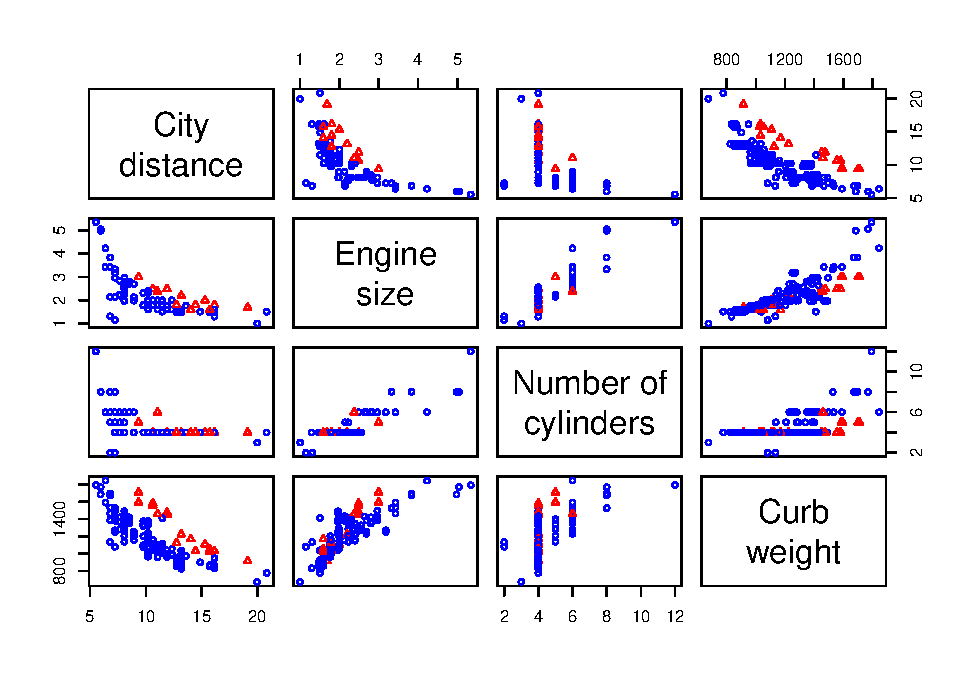
\includegraphics{fromBook_files/figure-latex/unnamed-chunk-1-1.pdf}

Some are qualitative:

\begin{itemize}
\tightlist
\item
  fuel type: diesel and gasoline
\end{itemize}

\textbf{We will in first phase consider only two explanatory variables:}

\begin{itemize}
\tightlist
\item
  Engine size, fuel type
\end{itemize}

To study the relationship between quantitative variables we usually make
a grafic representation.

\begin{Shaded}
\begin{Highlighting}[]
\CommentTok{### figure 2.2 }\AlertTok{###}
\KeywordTok{plot}\NormalTok{(engine.size, city.distance, }\DataTypeTok{type =} \StringTok{"n"}\NormalTok{, }\DataTypeTok{ylab =} \StringTok{"City distance (km/L)"}\NormalTok{,}
     \DataTypeTok{xlab =} \StringTok{"Engine size (L)"}\NormalTok{, }\DataTypeTok{xlim =} \KeywordTok{c}\NormalTok{(}\DecValTok{1}\NormalTok{, }\FloatTok{5.5}\NormalTok{))}
\KeywordTok{points}\NormalTok{(engine.size[d], city.distance[d], }\DataTypeTok{col =} \DecValTok{4}\NormalTok{, }\DataTypeTok{pch =} \DecValTok{1}\NormalTok{)}
\KeywordTok{points}\NormalTok{(engine.size[}\OperatorTok{!}\NormalTok{d], city.distance[}\OperatorTok{!}\NormalTok{d], }\DataTypeTok{col =} \DecValTok{2}\NormalTok{, }\DataTypeTok{pch =} \DecValTok{2}\NormalTok{)}
\KeywordTok{legend}\NormalTok{(}\StringTok{'topright'}\NormalTok{, }\DataTypeTok{pch =} \KeywordTok{c}\NormalTok{(}\DecValTok{1}\NormalTok{, }\DecValTok{2}\NormalTok{), }\DataTypeTok{col =} \KeywordTok{c}\NormalTok{(}\DecValTok{4}\NormalTok{, }\DecValTok{2}\NormalTok{),}
       \DataTypeTok{legend =} \KeywordTok{c}\NormalTok{(}\StringTok{"Gasoline  "}\NormalTok{,}\StringTok{"Diesel"}\NormalTok{))}
\end{Highlighting}
\end{Shaded}

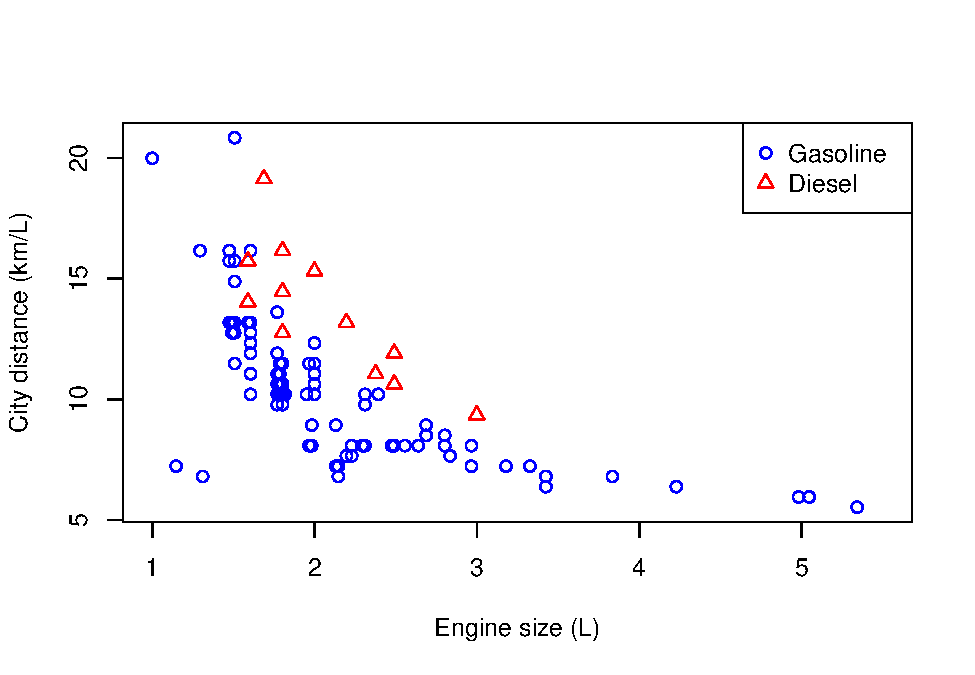
\includegraphics{fromBook_files/figure-latex/unnamed-chunk-2-1.pdf}

We first suggest a simple linear regression line:
\(y = \beta_{0} + \beta_{1} x + \epsilon\), where y represents city
distance, x fuel type, and \(\epsilon\) is a nonobservable random
`error', with expected value 0 and variance \(\sigma^2\). For simplicity
we consider no correlation between error terms and y. We need to find a
setimator for the unknown variales \(\beta_{0}\) and \(\beta_{1}\). To
do so wee need to user the method of least squares. Wich means the
finding the min of the function:

\center \(B(\beta)=\Sigma_{i=1}^n \{y_{i} -f(x_{i};\beta) \}^2 = ||y-f(x;\beta)||^2\)
\center

The last expressison is showing the matrix notation for representing
\(y = (y1,...,y_{n})^T; (f(x_{1};\beta),...,f(x_{m};\beta))^T;\).

\textbf{But from what we can see in the plot of `city distance against
engine size', a linear model might not be the best.} Therefor we might
consider a polynomial form, since it is easy and quick. The polynom will
look something like:
\center \(f(x;\beta) = \beta_{0} + \beta_{1} x + ... + \beta_{p-1} x^{p-1}\)
\center

Because of the simplicity if a polynomial we can wirte f in matrix form
with low effort, \center \(f(x;\beta)= X\beta\) \center where x is an n
x p matrix, called the design matrix, defined by
\cnter \(X=(1,x,...,x^{p-1})\) \center where x is the vector of the
observations of the explanatory variable, and the varius columns of X
contains powers of order from 0 to p-1 of elements of x.

On the matrix form the solution to the minimaztion problem is
\center \(\hat{\beta} = (X^{T}X)^{-1}X^{T}y\)

\hypertarget{computational-aspects}{%
\subsection{2.2 Computational Aspects}\label{computational-aspects}}

When we have alot of data the computation starts becomming important to
think about. And the main part of the calculation we need to look at is
the function

\center \(\hat{\beta} = (X^{T}*X)^{-1} X^{T} y\) \center (2.7)

\hypertarget{least-squares-estimation-by-successie-orthogonalization}{%
\subsubsection{2.2.1 Least Squares estimation by Successie
Orthogonalization}\label{least-squares-estimation-by-successie-orthogonalization}}

\end{document}
